% !TeX root = main.tex
\subsection{Evaluation Metrics}

We evaluate performance using two complementary metrics.

\paragraph{Maximum Cycle Count}
The maximum cycle count is the largest number of consecutive task cycles
completed before failure; higher values indicate better long-horizon
robustness.

\paragraph{Threading Tracking Error}
The threading tracking error measures the deviation of the observed thread from
its desired trajectory during execution; lower values indicate more accurate
tracking.

\subsection{Experimental Setup}

We evaluate the proposed method in both simulation and on real hardware using
the metrics defined above. Our platform comprises a seven-DoF Franka Research
3 (FR3) arm equipped with an Inspire Hand RH56DFX. Its simulated counterpart is
implemented in NVIDIA Isaac Sim~5.1.0 with Isaac Lab~2.2.1 and is used for
privileged teacher training, hybrid demonstration generation, and evaluation
before real-world transfer. The simulated and physical systems use the same
task geometry and OSC action interface.

In both settings, the student converts depth observations into cropped point
clouds and discards RGB. An Intel RealSense D415 supplies the physical RGB-D
stream. Real-world evaluation covers three nut sizes---M24, M30, and
M36---and four geometries per size: hexagonal, octagonal, rectangular, and
round.

% TODO: Validate and report the GPU, number of parallel environments, control
% and policy frequencies, camera calibration/resolution/frame rate,
% domain-randomization ranges, workspace and safety limits, trial counts,
% initialization distributions, and success/failure criteria.

\begin{figure}[t]
  \centering
  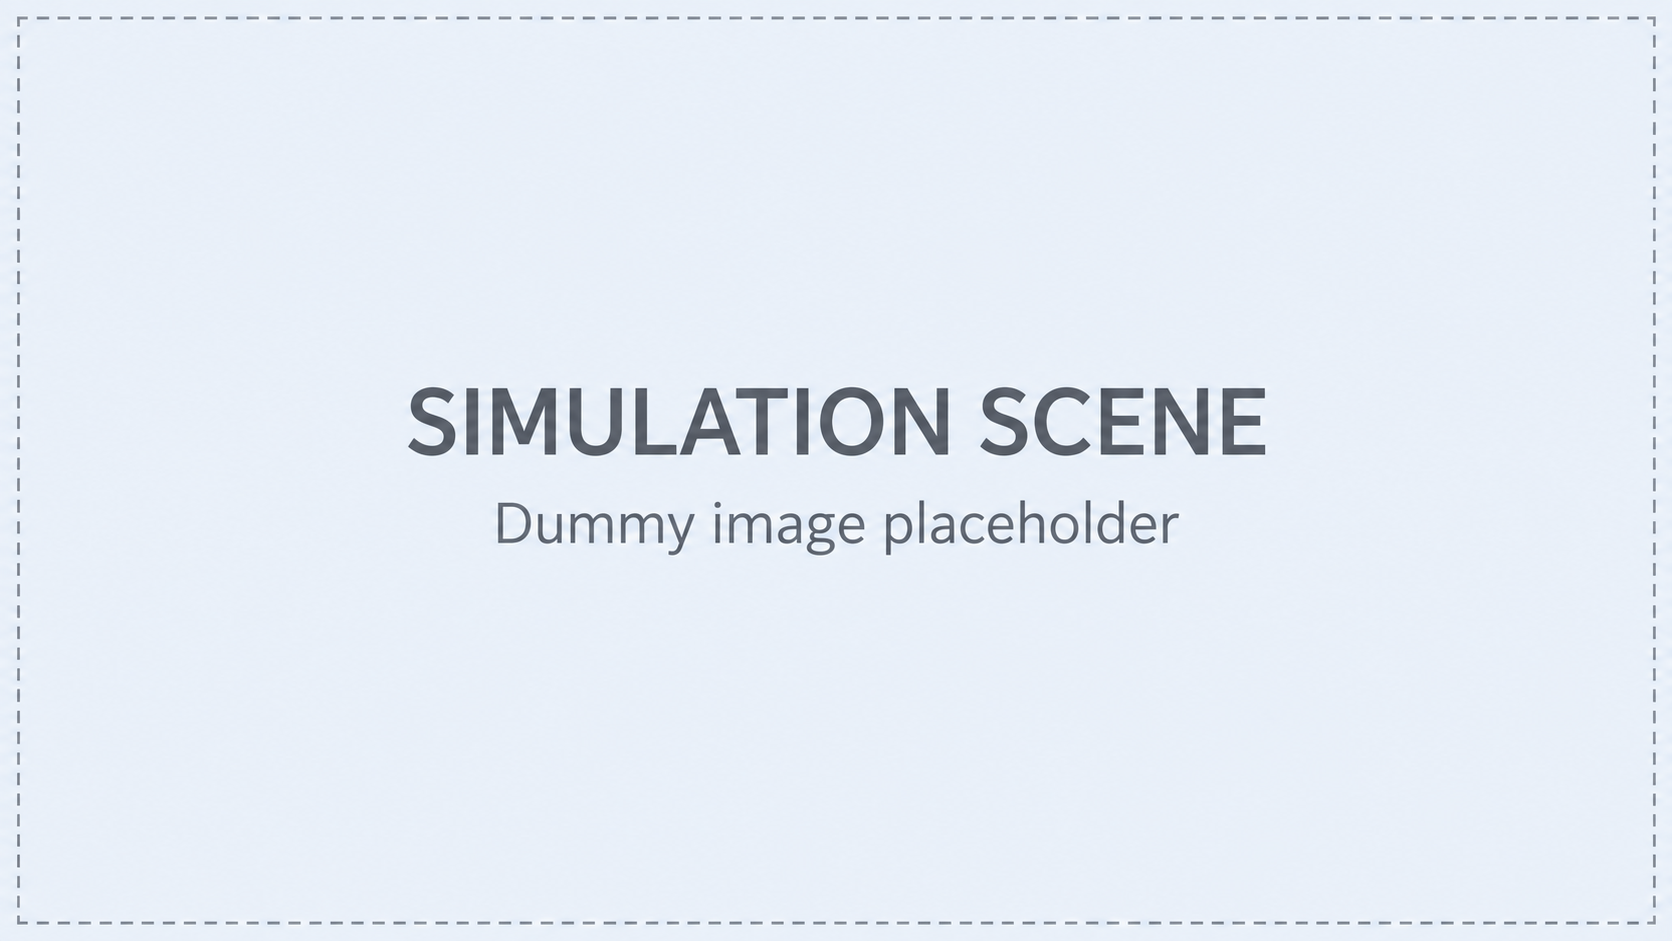
\includegraphics[width=\columnwidth]{figures/simulation_scene_placeholder.png}
  \caption{Simulation scene used for evaluation. Replace this placeholder with
    a representative view of the simulated robot, workspace, and threading
    task.}
  \label{fig:simulation_scene}
\end{figure}

\begin{figure}[t]
  \centering
  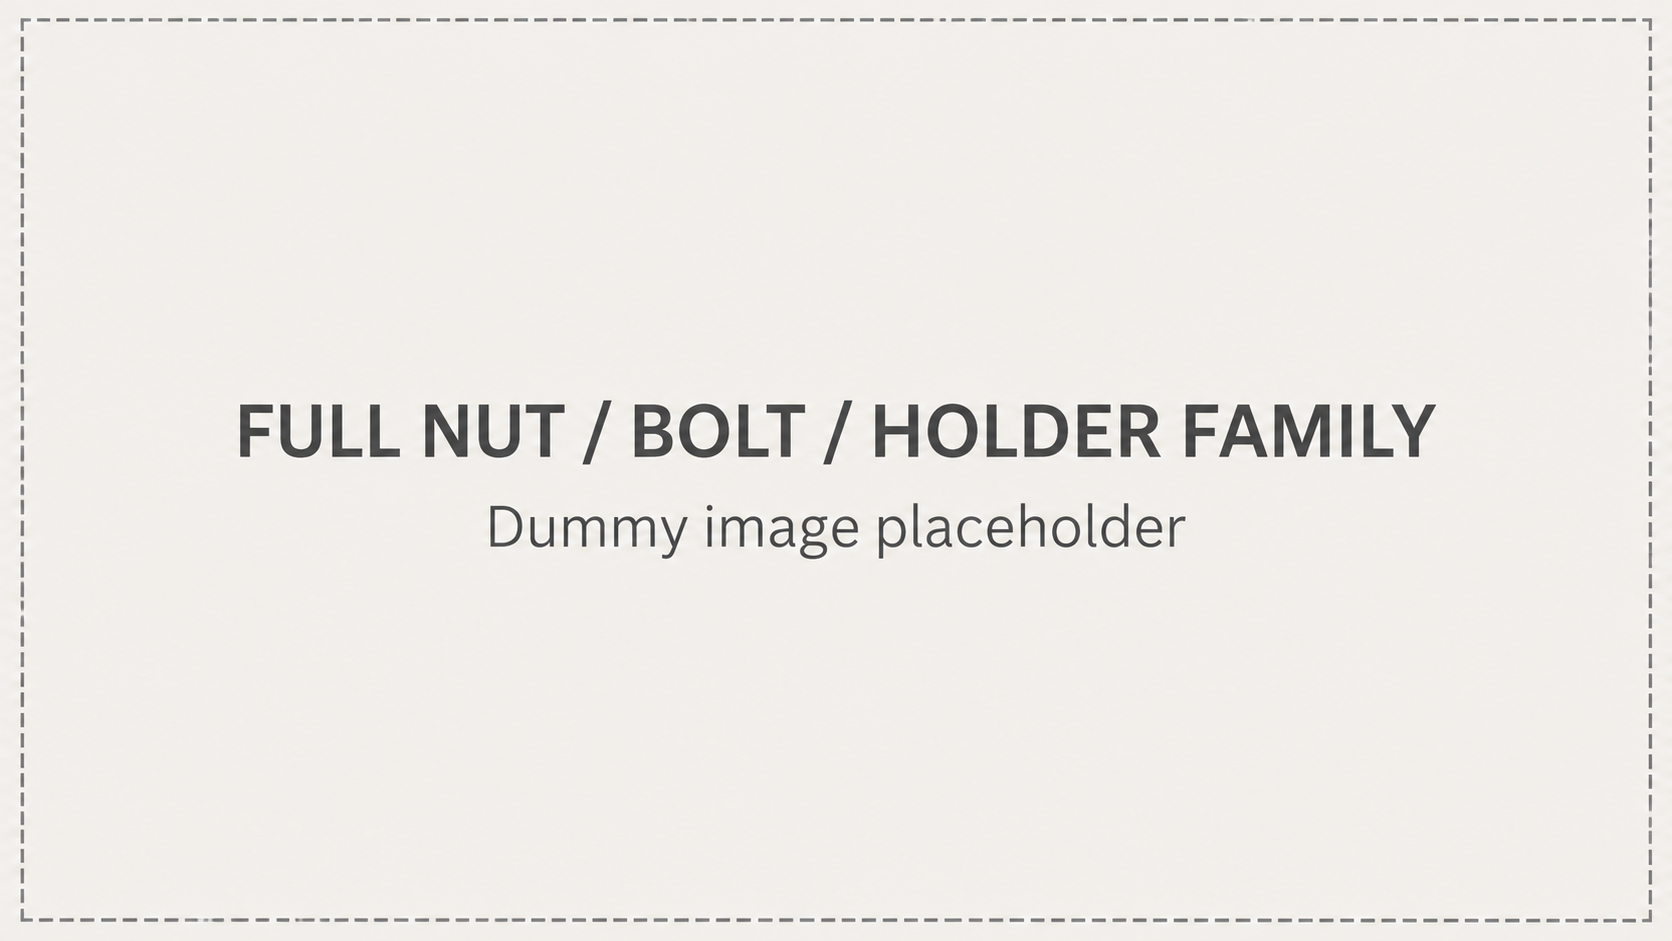
\includegraphics[width=\columnwidth]{figures/hardware_family_placeholder.png}
  \caption{Full family of nuts, bolts, and holders used in the real-hardware
    experiments. Replace this placeholder with a photograph showing all test
    objects and their geometric variations.}
  \label{fig:hardware_family}
\end{figure}

\subsection{Ablations}

We compare four policy-learning variants while keeping the architecture,
dataset budget, evaluation protocol, and all unrelated settings fixed.

\paragraph{Behavior Cloning}
Train the student policy using supervised behavior cloning on the initially
collected teacher demonstrations only.

\paragraph{Online DAgger}
Iteratively execute the current student policy, query the teacher online for
corrective actions on visited states, aggregate the new samples, and retrain the
student policy.

\paragraph{Offline DAgger}
Train on a fixed, pre-collected dataset that includes teacher corrections for
states visited by an intermediate student policy, without additional online
interaction during final training.

\paragraph{Ours}
Train once on the fixed dataset of hybrid-expert demonstrations and offline
human corrections using the proposed flow-matching imitation objective; no
student rollouts or online relabeling are used during training.

\subsection{Quantitative Results}

\begin{table}[htbp]
  \caption{Maximum cycle count for each nut size and geometry. Higher is
    better. Replace dashes with measured values.}
  \label{tab:maximum_cycle_count}
  \centering
  \begin{tabular}{lccc}
    \toprule
    Geometry & M24 & M30 & M36 \\
    \midrule
    Hexagonal  & -- & -- & -- \\
    Octagonal  & -- & -- & -- \\
    Rectangular & -- & -- & -- \\
    Round      & -- & -- & -- \\
    \bottomrule
  \end{tabular}
\end{table}


\begin{table}[htbp]
  \caption{Threading tracking error for each nut size and geometry. Lower is
    better. Replace dashes with measured values and report the unit.}
  \label{tab:thread_tracking_error}
  \centering
  \begin{tabular}{lccc}
    \toprule
    Geometry & M24 & M30 & M36 \\
    \midrule
    Hexagonal  & -- & -- & -- \\
    Octagonal  & -- & -- & -- \\
    Rectangular & -- & -- & -- \\
    Round      & -- & -- & -- \\
    \bottomrule
  \end{tabular}
\end{table}


\begin{table}[htbp]
  \caption{Success rate (\%) for each nut size and geometry. Higher is better.
    Replace dashes with measured values.}
  \label{tab:success_rate}
  \centering
  \begin{tabular}{lccc}
    \toprule
    Geometry & M24 & M30 & M36 \\
    \midrule
    Hexagonal  & -- & -- & -- \\
    Octagonal  & -- & -- & -- \\
    Rectangular & -- & -- & -- \\
    Round      & -- & -- & -- \\
    \bottomrule
  \end{tabular}
\end{table}


Interpret the three comparisons instead of repeating table entries. Discuss
maximum cycle count, threading tracking error, and success rate together, and tie
every central claim to the corresponding table or statistical test.

\subsection{Qualitative and Real-World Results}

Use vector figures (PDF) when possible, and ensure plot text remains legible at
the final column width. Discuss failure cases rather than reporting only the
best outcomes in the quantitative tables.
